\chapter{Stochastic Parameterization Suite}
\label{stoch}

Physical parameterization schemes represent averages over unresolved,
subgrid-scale processes, and those averages necessarily 
fluctuate depending on the precise realization of subgrid-scale
fields.  Hence, physical parameterization schemes should include a random,
``stochastic'' component.  To represent this random contribution to
forecast error, ensemble prediction systems now routinely use stochastic
parameterization schemes.
Stochastic parameterization schemes have been shown to improve the
probabilistic skill of weather forecasts on short- and medium-length forecast
timescales 
\citep[e.g.][]{Be09,Be11,leutbecher2017stochastic}.
Less known, however, is the fact that stochastic parameterization schemes also have the
potential to reduce systematic model error 
\citep[e.g.][]{berner2017stochastic}.

The stochastic parameterization suite in WRF comprises a number of
stochastic parameterization schemes, targeted at representing different aspects 
of uncertainty (see Table \ref {stoch_table}). Generally, one or more random
perturbation fields are generated and used to perturb tendencies or
parameters in the physical parameterization schemes.
The random perturbation fields are characterized by spatial and temporal
correlations as well as an overall perturbation amplitude, which can be
prescribed by namelist parameters. Figure \ref{stoch_pattern}
provides an example for perturbation patterns with different spatial length-scales.

%--------------------------------------------------------------------------------------------
\begin{table}
\label{stoch_table}
\begin{center}
\caption{Stochastic parameterization suite}
\begin{tabular}{ | l | l | l |}
\hline
Scheme          & Name & Perturbations to \\ 
\hline
SPPT  & Stochastically perturbed    &  u-,v-,$\theta$- and $q_v$-tendencies from PBL\\
      & parameterization tendencies &  and convection scheme\\  \hline

SKEBS & Stochastic kinetic-energy   &  Full ($=$ physics + dynamics) \\
      & backscatter scheme          &  $u_{\rm rot}$-,$v_{\rm rot}$- and $\theta$- tendencies\\  \hline

SPP & Stochastically perturbed      &  Select parameters from PBL \\
    & parameterization scheme       &  and convective scheme\\  \hline

RPF & Random perturbation field     &  Creates perturbation pattern only;  \\
    &                               &  interface must be provided by user\\
\hline
\end{tabular}
\end{center}
\end{table}
%--------------------------------------------------------------------------------------------

The benefits of stochastic parameterization schemes are most evident in ensemble 
prediction systems, where the added ensemble diversity leads to more reliable 
ensemble spread and improved probabilistic forecast skill \citep[e.g.][]{Be15}.

%--------------------------------------------------------------------------------------------
\begin{figure}[h!]
  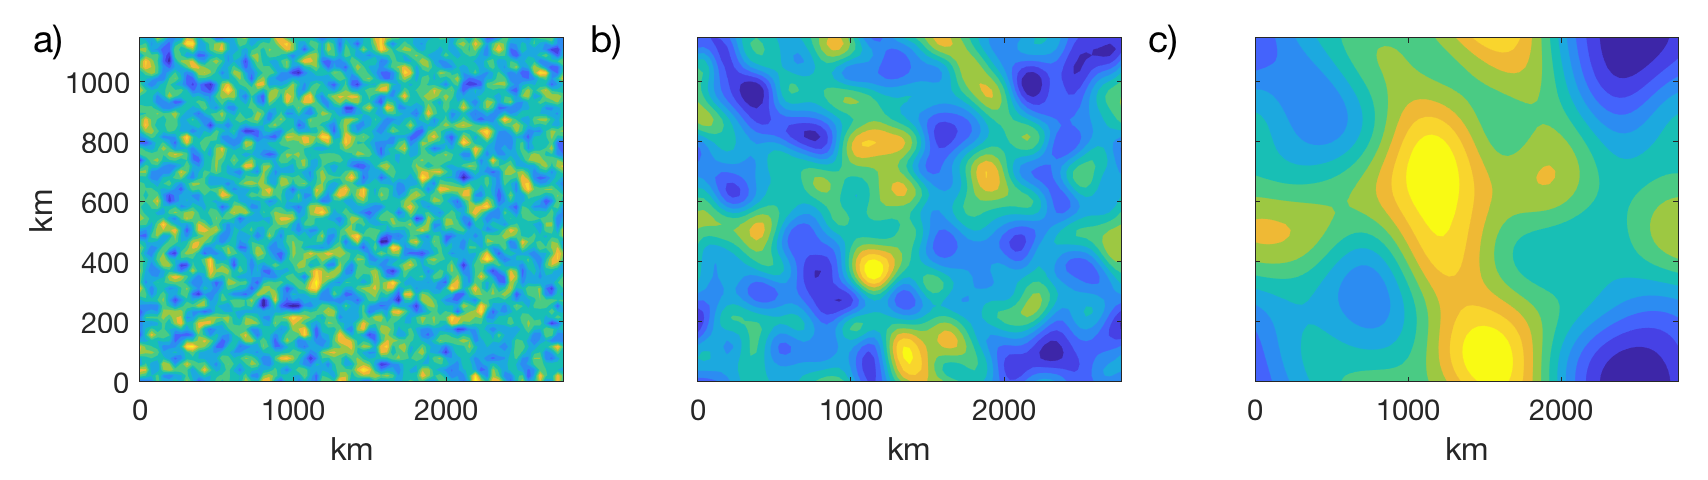
\includegraphics[width=6.5in]{figures/stoch_pattern.png}
    \caption{Perturbation patterns for three different spatial scales: 
     a) convection-scale, b) meso-scale, c) synoptic scale.}
  \label{stoch_pattern}
\end{figure}
%--------------------------------------------------------------------------------------------


%--------------------------------------------------------------------------------------------
\section {Stochastically Perturbed Physics Tendencies (SPPT)}
%--------------------------------------------------------------------------------------------
The Stochastically Perturbed Parameterization Tendency scheme
(SPPT) is based on the assumption that there is uncertainty
in the parameterized physics tendencies and that this 
uncertainty is proportional to the net physics tendency \citep{Bu99,Pa09}.
Consequently, SPPT perturbs the net physical tendency of temperature, 
humidity, and the wind components at each time step with a multiplicative 
random coefficient:
\begin{equation}
   \frac{\partial X}{\partial t}= D + (1+ r) \sum_i P_i \,.
\end{equation}
Here, ${\partial X}/{\partial t}$ denotes the total tendency in variable $X$, 
$D$ is the tendency from the dynamical core, 
$P_i$ the tendency from the i-th physics scheme, 
and $r$ is a two-dimensional, Gaussian distributed zero-mean random
perturbation field with spatial and temporal correlations (as in Fig.\, \ref{fig_stoch_pattern}).
Depending on
the implementation, the SPPT scheme can use up to three patterns with
different spatial and time scales, as well as a vertical tapering function which 
tapers perturbations near the surface and for the highest model levels.
The WRF implementation by default uses only a single perturbation field \citep{Be15},
and it perturbs the tendencies from the PBL and convection schemes, but not those from 
the radiation or microphysics schemes. For multiple domains, the perturbation pattern of the 
parent domain is interpolated to the nested domains.

%--------------------------------------------------------------------------------------------
\section{Stochastic Kinetic-Energy Backscatter Scheme (SKEBS)}
%--------------------------------------------------------------------------------------------
The Stochastic Kinetic Energy Backscatter scheme (SKEBS) aims to represent
the interactions of turbulent eddies near or below the
truncation level with the resolved state. Some of the eddy-eddy interactions
will dissipate, but others will lead to a resolved-scale effect.
Originally developed for large-eddy simulation applications, these ideas were 
adapted for numerical weather prediction by
\citet{Sh05} and \citet{Be09}.
SKEBS generates streamfunction perturbations with spatio-temporal
correlations, which perturb the rotational wind. These can be weighted
with the dissipation rate from numerical diffusion, convection, and
orographic wave drag.
In the WRF implementation, no dissipation weighting is used and the 
perturbations are extended to the potential temperature field \citep{Be11}.
Wind component perturbations are proportional to the square
root of the kinetic-energy backscatter rate, and temperature
perturbations are proportional to the potential energy backscatter rate.

A comparison of SKEBS and SPPT shows that SKEBS introduces the most model 
diversity in the free atmosphere and for dynamical variables, 
while SPPT is most active in regions with large tendencies (e.g., in areas with convection 
and near the surface) \citep{Be15}.
%--------------------------------------------------------------------------------------------
\section {Stochastically Perturbed Parameterization Scheme (SPP)}
%--------------------------------------------------------------------------------------------
To describe the statistics of the unresolved, subgrid-scale processes, 
physical parameterization schemes have a number of deterministic parameters.
While some of these have no uncertainty (e.g., the gravitational constant), 
others have large uncertainties due to 
measurement errors and heterogeneities in the underlying physical process.
Examples are the processes represented by the parameter ``roughness length'' in the PBL 
scheme or the shape parameter characterizing the particle size distribution in 
many microphysics schemes.  

The stochastically perturbed parameterization scheme (SPP)
perturbs the values of uncertain key parameters and thus provides 
a way to represent uncertainties within a particular parameterization scheme
\citep{Bo08,Ha11a}.
Perturbations in the convection scheme (e.g., to the vertical mass flux 
profile) or in the microphysics scheme (e.g., to the shape parameter of 
the particle size distribution) in principle allow the representation of
structural model error.  The statistical sciences fundamentally 
distinguish between ``parameter error'' and 
``structural error''. This distinction is blurred when some parameters in 
the physical schemes are perturbed, since parameter changes
can change the structural model error. Hence the scheme is referred to as 
``Stochastically perturbed \textit {parameterization} scheme'' rather than
``Stochastically perturbed \textit {parameter} scheme''. 

The SPP released in WRF has been designed in close collaboration with 
developers of physical parameterization and is under active development. 
Hence, it is only available for selected physics packages, namely the 
Grell-Freitas convection scheme and the MYNN PBL scheme \citep{jankov2017performance}.

The perturbations introduced by SPP tend to be smaller than those
introduced by SKEBS and SPPT and are by themselves typically not enough to
generate reliable ensemble spread \citep{Be15}.  However, SPP can be used 
to study forecast sensitivity to a particular parameter setting and/or
can be augmented by one of the other model-error schemes.

%--------------------------------------------------------------------------------------------
\section {Random Perturbation field (RPT)}
%--------------------------------------------------------------------------------------------
WRF enables the user to generate a 3-D Gaussian random perturbation field
with prescribed spatial and temporal correlations and use to it perturb
parameters or variables of interest. The interface to the perturbed quantity
has to be provided by the user. 

%--------------------------------------------------------------------------------------------
\section {Stochastic Perturbations to the Lateral Boundary Conditions}
%--------------------------------------------------------------------------------------------
The stochastic tendencies in WRF are typically treated as physics tendencies, and 
they change the perturbed fields at each time step within the WRF domain. However, since 
the stochastic perturbation field is also generated on the boundary, it can be used to 
perturb the lateral boundary specified and relaxation zones.
